\documentclass[a4paper,12pt]{report}
\usepackage{graphicx}
\pagestyle{myheadings}
\graphicspath { {'/'} }
\begin{document}
\author{Quang-Vinh Dang\\
COAST team - Inria}
\title{Technical Report: Performance measurement of Google Docs}\maketitle

\section{Introduction}
We want to evaluate the performance in term of delay with the collaborative editing service provided by Google\footnote{https://docs.google.com/}.
The delay is defined as: the time since an user (the sender) did a modification on his local Google Docs document (by using web browser) to the time since other users (the receivers) receive the modification on his local Google Docs document.
There are two parameters are using to control the measurement:
	\begin{itemize}
		\item The number of users who modify a document at the same time\footnote{Google claimed that Google Docs can support up to 50 users to modify at the same time. Visit https://support.google.com/drive/answer/2494827?hl=en for more details}.
		\item The typing speed of users, in term of how many character has been send from keyboard of user per second\footnote{The average typing speed in composition is about 20 word per minute, or around 2 characters per second. The information at http://en.wikipedia.org/wiki/Typing}.
	\end{itemize}
\section{Measurement settings}
The testing environment is: Ubuntu 14.10 64 bits\footnote{http://www.ubuntu.com/}.
The measurement is executed by using the following libraries and tools:
	\begin{itemize}
		\item Selenium\footnote{http://www.seleniumhq.org/}.
		\item xdotool\footnote{http://www.semicomplete.com/projects/xdotool/}.
	\end{itemize}
The result is processed by using:
	\begin{itemize}
		\item Python 2.7.+\footnote{https://www.python.org/}.
		\item R 3.1.2\footnote{http://www.r-project.org/}.
	\end{itemize}	 
To remove the difference in clock, the writing and reading users are simulated on a same computer. Other computers are used to simulate dummy writers.
\section{Result}
The result of the experiment is as Fig. \ref{fig:fig1}. \textit{u} means number of users, and \textit{s} means typing speed in term of how many character were typed per second.

	\begin{figure}
		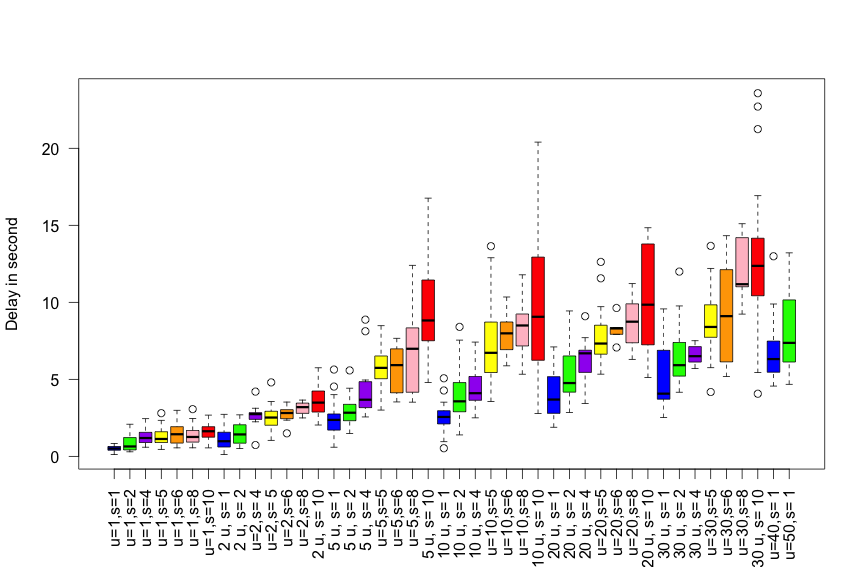
\includegraphics[width=\textwidth]{Rplot02}	
		\caption{Delays of Google Docs with different number of users and typing speed}
		\label{fig:fig1}
	\end{figure}

\section{Conclusion}
Google Docs is quite good for a small number of user with a slow typing speed (< 5 users and the typing speed is < 20 word per minute), but it does not work well with a large scale of user. We need some optimization and improvement to make the collaborative editing tool be suitable for a large scale of usage.
\end{document}